\chapter{Preliminares}\label{chapter02}

\section{Objetivo General}

Desarrollar\pdfcomment{Pongo un comentario acá pero porque no sé donde ponerlo. El título que aparece en el encabezado debe ser el mismo que aparece en la portada. Si llega a ser muy largo vemos como corregirlo} una plataforma web de predicción con inteligencia artificial para optimizar la producción diaria y reducir el desperdicio en comercios de productos perecederos, ajustando la oferta a la demanda real con base en datos históricos en el contexto de Buenos Aires 2025.\\

\noindent\textbf{Objetivos Específicos:}

\begin{itemize}
    \item Desarrollar un sistema de predicción de demanda diaria por producto utilizando inteligencia artificial, considerando variables como historial de ventas, día de la semana, clima y feriados.
    
    \item Implementar un módulo de carga y procesamiento automatizado de registros de venta, a partir de imágenes, mediante tecnologías de visión artificial y modelos de lenguaje.
    
    \item Diseñar una interfaz de backoffice con visualización de indicadores clave (KPIs), como márgenes, costos, productos más vendidos y ventas por franja horaria.
    
    \item Incorporar un asistente conversacional basado en lenguaje natural, que facilite la interacción del usuario con el sistema, permitiendo consultas operativas y recomendaciones automatizadas.
    
    \item Integrar un sistema de alertas y recomendaciones accionables, que anticipe sobreproducción o faltantes de stock y sugiera ajustes de planificación.
    
\end{itemize}

\section{Alcance}

El desarrollo de este producto de software será una aplicación web que incluirá las siguientes funcionalidades:

\begin{itemize}
    \item Se desarrollará un módulo de predicción de demanda diaria por producto, utilizando como variables de entrada el historial de ventas, día de la semana, clima y feriados, obteniendo como salida una predicción de producción del producto\pdfcomment{sobre la producción del producto}. 
    \item Incluirá\pdfcomment{Lo más correcto es decir "Se incluirá", lo mismo para los ítems siguientes} un dashboard que permita visualizar los KPIs más relevantes para la organización, tales como márgenes de ganancia, costos de insumos, productos más vendidos y visualización de ventas por franja horaria. 
    \item Implementará un chatbot que funcionará como interfaz principal de interacción con el sistema en el cual el usuario podrá realizar consultas.
    \item Implementará un sistema de carga de imágenes por parte del usuario, permitiendo subir registros de ventas directamente desde la interfaz web, extrayendo y almacenando automáticamente los datos desde las imágenes mediante LLMs.
    \item Se implementará un conjunto de alertas básicas automatizadas, que advertirán al usuario en casos de potencial sobreproducción o faltantes de stock antelación, en base a la comparación entre los valores proyectados y los datos de producción ingresados. 
    \item Se incorporará una herramienta de comparación de ventas semana a semana, que facilitará la identificación de patrones de comportamiento del consumo y permitirá evaluar la evolución del desempeño comercial en el tiempo.
\end{itemize}

\section{Antecedentes}

La investigación sobre predicción de demanda para productos perecederos ha avanzado con rapidez en los últimos años gracias a la IA. Modelos basados en LSTM y otras redes recurrentes superan sistemáticamente a los enfoques estadísticos clásicos al reducir tanto el exceso como la falta de stock en el comercio minorista alimentario (Nassibi et al., 2023) y demuestran mejoras similares en plataformas de “fresh food e-commerce” cuando se incorporan variables meteorológicas y calendarios (Ni et al., 2022)\pdfcomment{Orden cronológico}. Aun así, en Argentina se sigue desaprovechando el 12,5\% de la producción agroalimentaria, de las que solo el 1,2\% se pierden en la etapa comercial . El impacto se vuelve crítico en rubros como panaderías y pastelerías, donde en 2024 cerraron más de 400 locales y las ventas de pan cayeron un 53\%.

\newpage % <-- salto de página

\section{Marco Teórico}

En esta sección se describen los fundamentos conceptuales y técnicos necesarios para comprender el enfoque del sistema propuesto, incluyendo tecnologías de predicción, IA\pdfcomment{Inteligencia artificial pongan, las siglas IA recién la definen en la siguiente subsección}, aprendizaje automático y su aplicación en la predicción de demanda, y problemáticas sociales vinculadas al desperdicio de alimentos, que son relevantes para el sistema a desarrollar.


\subsection{Inteligencia Artificial (IA)}

La inteligencia artificial (en adelante IA) es un campo de estudio dentro de la informática que busca desarrollar sistemas capaces de realizar tareas que normalmente requieren inteligencia humana, tales como el razonamiento, la percepción, la toma de decisiones o el aprendizaje. El término fue acuñado formalmente en 1956 durante la conferencia de Dartmouth, considerada el punto de partida de la disciplina \parencite{mccarthy1955}.\\

En términos generales, la IA puede dividirse en dos grandes enfoques:

\begin{itemize}
    \item \textbf{IA débil} (\textit{narrow AI}): especializada en tareas concretas como traducción automática, recomendación de productos o reconocimiento de imágenes.
    
    \item \textbf{IA fuerte} (\textit{general AI}): de carácter hipotético, orientada a replicar el razonamiento humano en su totalidad \parencite{russell2021}\pdfcomment{Está raro que solo este la cita para este ítem. Debería ser uno solo para ambos, o una referencia para cada uno}.
\end{itemize}

Gracias al aumento en la capacidad de cómputo y al acceso a grandes volúmenes de datos, el desarrollo reciente de IA basada en aprendizaje automático (\textit{machine learning}) ha permitido avances significativos en múltiples industrias, incluyendo salud, finanzas, logística y comercio minorista \parencite{jordan2015}.

Estos avances han dado lugar al uso extendido de IA en tareas de predicción de demanda, optimización de recursos y automatización de procesos, tal como se propone en el presente proyecto.

La IA también se ha convertido en una herramienta clave para abordar problemáticas socioambientales, como el desperdicio de alimentos, al permitir el análisis en tiempo real de patrones de consumo y la generación de alertas y recomendaciones \parencite{rolnick2019}.

\subsection{Aprendizaje Automático}

El aprendizaje automático (\textit{machine learning}, en adelante ML) es una subárea de la inteligencia artificial que se enfoca en desarrollar algoritmos capaces de aprender automáticamente a partir de datos, identificar patrones y realizar predicciones o tomar decisiones sin ser programados explícitamente para cada tarea específica \parencite{mitchell1997}.

En contraste con la programación tradicional —donde se define explícitamente cada regla—, en ML los sistemas ajustan su comportamiento a partir de ejemplos y experiencia previa, lo que permite adaptarse a entornos dinámicos o impredecibles. Existen tres grandes categorías de aprendizaje automático:

\begin{itemize}
    \item \textbf{Supervisado}: el modelo se entrena con datos etiquetados\pdfcomment{definir en una oración qué es un dato etiquetado, justo antes de este ítem, o bien, con el comando footnote} (por ejemplo, ventas históricas con cantidades reales).
    
    \item \textbf{No supervisado}: busca patrones o agrupamientos en datos no etiquetados.
    
    \item \textbf{Por refuerzo}: el agente aprende mediante recompensas o penalizaciones por sus acciones \parencite{sutton2018}\pdfcomment{idem mi comentario sobre referencias en el itemize anterior}.
\end{itemize}

En el ámbito de la predicción de demanda y la gestión comercial, el ML ha demostrado ser altamente efectivo. Algoritmos como regresiones, árboles de decisión, \textit{random forest}, redes neuronales o XGBoost permiten prever comportamientos complejos en entornos de alta variabilidad, como el retail alimentario o los productos perecederos \parencite{carbonneau2008}.

Gracias a su capacidad para adaptarse a datos históricos y variables externas —como el clima, promociones o eventos locales—, el ML se ha convertido en una herramienta estratégica para reducir mermas, optimizar la producción y tomar decisiones basadas en evidencia, alineándose con los objetivos del presente proyecto.

\subsection{Series Temporales}

Una serie temporal es una secuencia de observaciones recolectadas en intervalos regulares a lo largo del tiempo. Este tipo de datos permite analizar la evolución de un fenómeno y modelar su comportamiento futuro mediante técnicas estadísticas o de aprendizaje automático \parencite{chatfield2004}. En el caso del comercio minorista, las ventas históricas diarias o semanales de un producto conforman una serie temporal típica.\\

Las series temporales suelen contener tres componentes principales:

\begin{itemize}
    \item \textbf{Tendencia (trend)}: dirección general del movimiento a largo plazo.
    
    \item \textbf{Estacionalidad (seasonality)}: patrones repetitivos dentro de un periodo (como días de la semana o estaciones).
    
    \item \textbf{Ruido (noise)}\pdfcomment{En uno de los itemize anterior usaron italic para el texto entre paréntisis y acá usar bf, elijan uno de los dos y mantengan el formato cada vez que les aparezca algo así}: variaciones aleatorias e impredecibles.
\end{itemize}

La predicción de series temporales es crucial para aplicaciones como la planificación de la producción, gestión de inventarios y optimización de recursos, ya que permite anticiparse a picos o caídas en la demanda \parencite{hyndman2018}.

Tradicionalmente, se utilizaron modelos como ARIMA, Holt-Winters y modelos exponenciales suavizados, aunque en la actualidad han ganado terreno los modelos basados en aprendizaje automático y redes neuronales, especialmente cuando se incorporan variables exógenas como el clima o eventos especiales \parencite{bandara2020}.

En el presente proyecto, las series temporales constituyen la estructura central sobre la cual se apoyará la generación de predicciones de demanda, mediante el uso de modelos ya existentes y herramientas que permiten adaptarse dinámicamente a los patrones observados en los datos históricos y en el contexto operativo del comercio.

\subsection{Modelos de Predicción}

Los modelos de predicción son herramientas matemáticas o computacionales que permiten estimar el valor futuro de una variable en función de sus observaciones pasadas y/o de otras variables relacionadas. En el contexto de series temporales, estos modelos se utilizan para anticipar comportamientos futuros de fenómenos que evolucionan en el tiempo, como la demanda de productos perecederos en comercios minoristas \parencite{hyndman2018}.

Entre los enfoques tradicionales más utilizados se encuentran:

\begin{itemize}
    \item \textbf{Regresión lineal}\pdfcomment{Regresión lineal es un caso particular de la Regresión. Creo que es mejor que definan Regresión, y pueden mantener parte del texto explicando cómo funciona la que es lineal.}: técnica estadística básica que modela la relación entre una variable dependiente y una o más variables independientes. Es útil en escenarios con relaciones simples y datos bien estructurados, aunque su capacidad para capturar patrones no lineales es limitada.
    
    \item \textbf{ARIMA (AutoRegressive Integrated Moving Average)}: combina componentes autorregresivos, de promediado móvil y diferenciación para tratar series no estacionarias \parencite{box2015}.
    
    \item \textbf{Holt-Winters}: extensión del suavizado exponencial que incorpora estacionalidad y tendencia, útil para pronósticos a corto plazo con ciclos estables.
\end{itemize}

Estos modelos son apreciados por su simplicidad y bajo costo computacional, aunque presentan limitaciones cuando hay muchas variables externas o relaciones no lineales.

Con el auge del aprendizaje automático, se han incorporado técnicas más complejas que permiten capturar relaciones no lineales y variables exógenas:

\begin{itemize}
    \item \textbf{Prophet}: modelo desarrollado por Facebook que permite ajustar estacionalidades múltiples y eventos especiales de forma flexible \parencite{taylor2018}.
    
    \item \textbf{LSTM (Long Short-Term Memory)}: tipo de red neuronal recurrente capaz de aprender dependencias de largo plazo, muy utilizada en predicción de series temporales con datos ruidosos o variables múltiples \parencite{hewamalage2021}\pdfcomment{Quedó mal esta referencia}.
\end{itemize}

Como se observa en la Figura~\ref{fig:lstm}, esta arquitectura permite mantener y transmitir información a lo largo del tiempo, lo cual la hace especialmente útil para modelar secuencias con relaciones temporales complejas.

\begin{figure}[t]
    \centering
    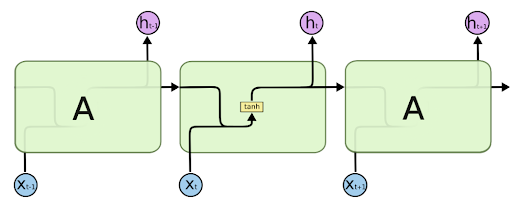
\includegraphics[width=0.7\textwidth]{images/lstm.png}
    \caption{LSTM (Long Short-Term Memory) básico.}
    \label{fig:lstm}
\end{figure}

\begin{itemize}
    \item \textbf{Transformers}: arquitectura inicialmente desarrollada para procesamiento de lenguaje natural, que ha comenzado a aplicarse con éxito en predicción multivariada de series temporales \parencite{li2019}.
\end{itemize}

La elección del modelo dependerá del tipo de datos disponibles, la granularidad deseada y los requisitos de interpretabilidad y precisión. En este proyecto, estos modelos permitirán estimar con mayor exactitud la demanda diaria de productos, reduciendo mermas y ajustando la producción a las condiciones reales del entorno.

\subsection{Evaluación de Modelos Predictivos}

La evaluación de modelos predictivos es un paso fundamental en el desarrollo de soluciones basadas en inteligencia artificial o series temporales, ya que permite medir cuán precisas y útiles son las predicciones generadas. Para problemas de regresión —como la predicción de demanda— se utilizan principalmente métricas de error que comparan los valores predichos con los observados.

Entre las más utilizadas se encuentran:

\begin{itemize}
    \item \textbf{MAE (Mean Absolute Error)}: mide el promedio de los errores absolutos entre las predicciones $\hat{y}_t$ y los valores reales $y_t$ \parencite{willmott2005}.
    
    \[
        \text{MAE} = \frac{1}{n} \sum_{t=1}^{n} \left| y_t - \hat{y}_t \right|
    \]

    \item \textbf{RMSE (Root Mean Squared Error)}: calcula la raíz cuadrada del promedio de los errores al cuadrado, penalizando más fuertemente los errores grandes \parencite{chai2014}.
    
    \[
        \text{RMSE} = \sqrt{ \frac{1}{n} \sum_{t=1}^{n} \left( y_t - \hat{y}_t \right)^2 }
    \]

    \item \textbf{MAPE (Mean Absolute Percentage Error)}: expresa el error como un porcentaje del valor real. Es útil para comparar modelos en distintas escalas, aunque puede ser inestable cuando $y_t \approx 0$ \parencite{myttenaere2016}.
    
    \[
        \text{MAPE} = \frac{100}{n} \sum_{t=1}^{n} \left| \frac{y_t - \hat{y}_t}{y_t} \right|
    \]
\end{itemize}

La elección de la métrica depende del contexto. El MAE es más interpretable para usuarios no técnicos, mientras que el RMSE resulta más sensible a errores significativos. En el caso de predicción de demanda para comercios de productos perecederos, se recomienda utilizar al menos dos métricas para una evaluación equilibrada.\pdfcomment{¿Quién recomienda? Si saben, pongan la referencia, si no, quiten esta oración, o digan cuál van a usar y por qué}

Estas herramientas también permiten monitorear el desempeño del modelo en producción, facilitando el mantenimiento de su precisión a lo largo del tiempo.

\subsection{Reconocimiento Óptico de Caracteres (OCR)}

\indent El Reconocimiento Óptico de Caracteres (OCR) es una tecnología que permite convertir texto impreso o manuscrito en imágenes digitales en texto editable y procesable por máquinas. Es ampliamente utilizada en tareas como la digitalización de documentos, la lectura automatizada de facturas, tickets, formularios y libros (Smith, 2007)\pdfcomment{Hay varias referencias como estas que no están referencias con LaTeX. Tienen que hacerlo porque si no la bibliografía puede no coincidir con el texto}.

\indent Inicialmente, los sistemas OCR se basaban en técnicas de procesamiento de imágenes y plantillas estáticas, lo que limitaba su capacidad para adaptarse a diferentes formatos, caligrafías o niveles de ruido. Sin embargo, los avances en aprendizaje profundo han revolucionado esta tecnología: los modelos actuales, como CRNN (Convolutional Recurrent Neural Network) y los basados en transformers como TrOCR, ofrecen una mayor precisión y robustez en entornos no estructurados, como fotos tomadas con teléfonos móviles o documentos parcialmente dañados (Baek et al., 2019; Li et al., 2021).

\indent El OCR es especialmente valioso en contextos donde los usuarios no pueden o no desean realizar carga manual de datos, como en pequeños comercios. Al automatizar la lectura de registros de venta o remitos mediante fotos, se reduce la carga operativa y se mejora la calidad del dato ingresado (Khandelwal et al., 2020).

\indent En este proyecto, el OCR cumple un rol clave al permitir a los comerciantes digitalizar información histórica de ventas sin conocimientos técnicos, usando simplemente una fotografía desde la plataforma web, lo cual democratiza el acceso a herramientas de predicción.


\subsection{Modelos de Lenguaje Extensos (LLM)}

\indent Los Modelos de Lenguaje Extensos (Large Language Models, LLM) son un tipo avanzado de modelo de IA entrenado con enormes cantidades de texto para comprender, generar y manipular lenguaje natural de forma coherente y contextual. Se basan en arquitecturas como transformers, que han demostrado ser altamente eficaces para tareas complejas de procesamiento del lenguaje natural (Vaswani et al., 2017).

\indent Los LLM aprenden a predecir la siguiente palabra en una secuencia, lo que les permite ejecutar tareas como generación de texto, traducción, resumen automático, respuestas a preguntas y análisis semántico. Modelos como GPT-3, PaLM, BERT o LLaMA han alcanzado niveles de rendimiento cercanos al humano en una variedad de benchmarks lingüísticos (Brown et al., 2020; OpenAI, 2023).

\indent Una de las aplicaciones emergentes de los LLM es su integración con otros flujos de datos no estructurados, como imágenes o documentos escaneados, lo que los convierte en una herramienta poderosa para la automatización de tareas que antes requerían intervención humana. En combinación con OCR y pipelines de extracción, los LLM pueden interpretar textos ambiguos, corregir errores y convertir inputs visuales en información estructurada\pdfcomment{Esto me hace ruido. La información se almacena en forma de tensores, pero no sé si esto cae dentro de la categoría de estructuradas. Update: estaba leyendo más abajo y efectivamente mencionan que es no estructurada, así que esto está mal} (Touvron et al., 2023).

\indent En el contexto de este proyecto, los LLM permiten automatizar la carga de registros de ventas a partir de imágenes, interpretar consultas del usuario en lenguaje natural a través de un chatbot y ofrecer respuestas explicativas, todo sin requerir conocimientos técnicos del usuario final.

\subsection{Chatbots Conversacionales}

Los chatbots conversacionales son sistemas informáticos diseñados para interactuar con los usuarios mediante lenguaje natural, ya sea por texto o voz. Su objetivo principal es simular una conversación humana para asistir, informar, resolver consultas o ejecutar acciones específicas dentro de una plataforma digital \parencite{radziwill2017}.

Originalmente basados en reglas fijas y árboles de decisión, los chatbots han evolucionado significativamente gracias a los avances en procesamiento de lenguaje natural (PLN), generación de lenguaje natural (GNL\pdfcomment{Es GLN, o en inglés NLG, pero GNL no. Corríjanlo en todos los lugares donde esto pase}) y, más recientemente, en modelos de lenguaje extensos (LLM\pdfcomment{LLM es la única sigla que la tienen en inglés. Aclaren en algún lugar que sus siglas vienen del inglés. No las pongan en español porque LLM es usado en español también y conviene mantenerlo}). Estas tecnologías les permiten comprender intenciones\pdfcomment{y entidades. No aclaren que significa pero se los comento porque tienen que saberlo: una entidad es algo a detectar en un texto. Por ejemplo, si trato de conocer la dirección de un lugar, la dirección sería una entidad. Alguien puede decirme la dirección de una forma no muy prolija, pero el modelo sería capaz de entenderlo igual. Hasta cierto límite, porque estos modelos no son muy buenos con razonamientos puros,por lo que si le haces razonar para llegar a la solución probablemente fallaría por eso, pero no por la entidad. Igualmente hay una probabilidad de falla para la entidad pero es demasiado baja, y es por eso que por ejemplo GPT da cosas tan coherentes}, responder con mayor coherencia y adaptarse al contexto de las interacciones \parencite{shum2018}.

Existen distintos tipos de chatbots, entre ellos:

\begin{itemize}
    \item \textbf{Chatbots basados en reglas}: operan sobre flujos de conversación predefinidos.
    
    \item \textbf{Chatbots con IA}: utilizan algoritmos de aprendizaje automático, PLN y GNL para entender y generar respuestas dinámicas.
    
    \item \textbf{Chatbots híbridos}: combinan ambos enfoques, lo que los hace flexibles y eficientes.
\end{itemize}

En aplicaciones empresariales, los chatbots se utilizan cada vez más para consultas sobre datos, gestión de operaciones y soporte a decisiones, especialmente en entornos con usuarios no técnicos. Estudios recientes demuestran que la incorporación de asistentes conversacionales mejora la adopción de sistemas analíticos complejos, reduce barreras de entrada y mejora la experiencia del usuario \parencite{knote2021}.

En este proyecto, el chatbot actuará como interfaz principal del sistema, permitiendo al comerciante consultar predicciones de demanda, indicadores clave (KPIs\pdfcomment{Anoten para no olvidarnos que esto estaría bueno que aparezca a un costado del chat}), alertas de sobreproducción y sugerencias de acción, sin necesidad de navegar por menús complejos ni interpretar gráficos técnicos.

\subsection{Bases de Datos Relacionales y Vectoriales}

Las bases de datos relacionales (RDB, por sus siglas en inglés\pdfcomment{Este formato es con el que deben explicar las siglas LLM}) son estructuras de almacenamiento que organizan la información en tablas con filas y columnas, siguiendo un modelo basado en el álgebra relacional, propuesta por Edgar F. Codd en 1970. Este modelo formaliza las operaciones sobre conjuntos de datos utilizando el concepto de relación, y se convirtió en el estándar dominante para almacenar información estructurada en sistemas informáticos \parencite{codd1970}. 

Las bases relacionales permiten realizar consultas complejas mediante lenguajes como SQL y son ampliamente utilizadas en aplicaciones empresariales debido a su robustez, integridad referencial y facilidad de acceso \parencite{coronel2020}.

En contraposición, las bases de datos vectoriales son un tipo más reciente de almacenamiento orientado a datos no estructurados o semiestructurados representados como tensores. Su principal aplicación está en sistemas que utilizan inteligencia artificial, especialmente modelos de lenguaje, visión por computadora y recuperación semántica, donde se requiere comparar elementos no por igualdad exacta, sino por similitud de contexto o significado \parencite{johnson2019}.

Estos vectores se obtienen comúnmente a través de \textit{embeddings} generados por modelos como Word2Vec, BERT o CLIP, y se almacenan en motores especializados como FAISS, Milvus o Pinecone, optimizados para búsquedas por proximidad (\textit{nearest neighbor search}).

En el contexto de este proyecto, las bases relacionales serán utilizadas para almacenar información estructurada como productos, ventas, fechas y predicciones, mientras que las bases vectoriales podrían emplearse en versiones futuras para mejorar el rendimiento del chatbot, permitiéndole recuperar respuestas basadas en similitud semántica entre preguntas y registros históricos o documentación del sistema.

\subsection{Desperdicio de Alimentos}

El desperdicio de alimentos hace referencia a la pérdida de productos aptos para el consumo humano que son descartados, deteriorados o no utilizados en etapas finales de la cadena alimentaria, como la comercialización, el almacenamiento o el consumo doméstico. Se diferencia de la pérdida de alimentos, que ocurre en fases anteriores como la producción, poscosecha o procesamiento \parencite{fao2019}\pdfcomment{Esta cita está rara}.

A nivel mundial, se estima que alrededor del 17\% de los alimentos disponibles para los consumidores se desperdicia, lo que representa no solo un problema ético y de seguridad alimentaria, sino también una amenaza ambiental por el uso innecesario de recursos como agua, tierra y energía, y la generación de gases de efecto invernadero \parencite{unep2021}.

En Argentina, se pierde o desperdicia el 12{,}5\% de la producción agroalimentaria, lo que equivale a aproximadamente 16 millones de toneladas por año, con consecuencias económicas directas para todos los actores de la cadena de valor \parencite{tiscornia2022}. Particularmente en supermercados, autoservicios y comercios de proximidad, estudios recientes estiman que las pérdidas en categorías frescas superan el 3\% de la facturación, debido a sobreproducción, quiebres de stock, manipulación inadecuada o falta de planificación \parencite{weteam2021}.

Estas cifras revelan la importancia de implementar soluciones basadas en inteligencia artificial y analítica de datos para alinear la producción con la demanda real, evitar el sobrante no comercializable y aumentar la eficiencia operativa. Además, el combate al desperdicio de alimentos contribuye directamente al cumplimiento del Objetivo de Desarrollo Sostenible (ODS) 12: Producción y Consumo Responsables, propuesto por la ONU para 2030.

\subsection{Impacto Económico del desperdicio de alimentos}

El desperdicio de alimentos no solo representa una pérdida de recursos naturales y energéticos, sino también un impacto económico significativo para productores, distribuidores, comercios y consumidores. En cada etapa de la cadena alimentaria, los alimentos descartados implican costos hundidos en insumos, mano de obra, energía, logística y espacio, sin retorno económico alguno \parencite{gustavsson2011}.

A nivel global, se estima que el valor económico del desperdicio asciende a 1 billón de dólares anuales, afectando tanto a países desarrollados como en desarrollo \parencite{fao2013}\pdfcomment{Las citas así largas, estoy casi seguro que están mal}. En entornos urbanos y comerciales, las pérdidas se concentran especialmente en productos frescos y perecederos —como panificados, frutas, carnes y lácteos— debido a errores de planificación, sobreproducción, fluctuaciones de demanda o una gestión ineficiente de inventarios \parencite{fao2019}.

En Argentina, estudios sectoriales revelan que las pérdidas en supermercados y autoservicios superan el 3\% de la facturación en categorías de frescos y almacén, representando un margen crítico para negocios con alta rotación y baja rentabilidad unitaria \parencite{weteam2021}. En comercios pequeños, como panaderías y pastelerías, esta ineficiencia se ve agravada por la falta de herramientas analíticas y predictivas que permitan anticipar la demanda real, provocando mermas frecuentes y subutilización de insumos.

El impacto económico también afecta a escala sistémica: cada tonelada de alimento desperdiciado implica no solo una pérdida directa, sino también costos ocultos en la cadena logística, residuos, tratamiento y emisiones \parencite{refed2016}. Desde esta perspectiva, el desarrollo de soluciones tecnológicas que minimicen el desperdicio contribuye no solo a mejorar la rentabilidad del negocio, sino también a reducir costos operativos y ambientales a largo plazo.

\subsection{Impacto Ambiental del Desperdicio de Alimentos\pdfcomment{Acá tienen las iniciales en mayúsculas y en la anterior en minúscula. Además, creo que es redundante el "del desperdicio de alimentos", porque es el nombre de esta sección}}

El desperdicio de alimentos tiene consecuencias ambientales severas, ya que cada unidad de alimento producida pero no consumida implica un uso innecesario de recursos naturales, como agua, suelo y energía, además de generar residuos y emisiones contaminantes. La huella ambiental del desperdicio incluye tres grandes dimensiones: la huella hídrica, la huella de carbono y el uso del suelo \parencite{fao2013}.

A nivel mundial, se calcula que el desperdicio de alimentos genera entre el 8\pdfcomment{Símbolo de porcentaje también acá. Se que lo podría escribir yo, pero mi idea es que aprendan cuál es el error además de que no debería meter mano en el texto final, solo dar recomendaciones} y el 10\% de las emisiones globales de gases de efecto invernadero (GEI), lo que equivale a más de 3.300 millones de toneladas de CO\textsubscript{2} emitidas anualmente \parencite{unep2021}. Si el desperdicio de alimentos fuera un país, sería el tercer mayor emisor del mundo, detrás de China y Estados Unidos \parencite{fao2013}\pdfcomment{Esta referencia está muy atrás en el tiempo. Para ese momento también entre el 8\% y el 10\%? Si no logran averiguarlo, reestructuren el párrafo sin este dato}.

En cuanto a recursos hídricos, se estima que alrededor de 250~km\textsuperscript{3} de agua se utilizan cada año para producir alimentos que nunca serán consumidos, lo que representa una presión significativa sobre acuíferos y sistemas hídricos vulnerables. Además, el uso ineficiente del suelo para cultivos que luego se pierden contribuye a la deforestación, pérdida de biodiversidad y degradación de ecosistemas \parencite{kummu2012}.

En el caso de Argentina, donde se desperdician más de 16 millones de toneladas de alimentos por año \parencite{tiscornia2022}, el impacto ambiental se agrava por la dependencia del sector agroindustrial como motor económico, lo que exige soluciones que equilibren productividad y sostenibilidad. Reducir el desperdicio, por tanto, no solo mejora la eficiencia de los sistemas alimentarios, sino que también representa una estrategia concreta de mitigación del cambio climático \parencite{unep2021}.

Desde esta perspectiva, el proyecto presentado cobra relevancia al buscar reducir la sobreproducción mediante herramientas de predicción basadas en inteligencia artificial, contribuyendo así a una gestión más sostenible de los recursos.

\subsection{ODS 12 – Producción y Consumo Responsables\pdfcomment{Es raro que utilicen un guión en el título de una sección. Quizás sea mejor poner solo ODS 12 y luego aclarar más abajo que es.}}

El Objetivo de Desarrollo Sostenible 12 (ODS 12), propuesto por las Naciones Unidas en la Agenda 2030, tiene como meta garantizar modalidades de consumo y producción sostenibles, promoviendo un uso eficiente de los recursos, la energía y los sistemas productivos, sin comprometer las necesidades de las generaciones futuras \parencite{onu2015}.

Uno de los ejes centrales del ODS 12 es la reducción sustancial del desperdicio de alimentos, tanto en la etapa de producción como en los sectores minorista y de consumo. La meta 12.3, en particular, establece como compromiso internacional reducir a la mitad el desperdicio de alimentos per cápita mundial en el comercio minorista y el consumidor para el año 2030, y disminuir las pérdidas a lo largo de las cadenas de producción y suministro \parencite{unep2021}.\pdfcomment{Esto parece algo que se podría citar textual. En caso de hacerlo, pongan algo así como "citando textualmente: ...", y lo que necesitan entre comillas luego de los dos puntos}

Este objetivo reconoce que el desperdicio alimentario es un problema transversal: tiene impactos económicos, sociales (inseguridad alimentaria) y ambientales (emisiones de gases de efecto invernadero, uso de agua y suelo). Por eso, la tecnología juega un rol clave como habilitadora de soluciones innovadoras y escalables, particularmente en el sector privado.

En este contexto, el presente proyecto de ingeniería se alinea directamente con el ODS 12, al proponer una plataforma que utiliza inteligencia artificial para predecir la demanda real en comercios de productos perecederos, evitando sobreproducción y mermas innecesarias. Así, no solo mejora la rentabilidad de los negocios, sino que contribuye a un modelo de producción más eficiente, consciente y responsable con el entorno.

\subsection{Digitalización y brecha tecnológica en PYMEs}

\pdfcomment{Esta sección no estoy seguro de si debería ir. El público objetivo no eran comercios? caen dentro del concepto de PYME?} La digitalización implica la incorporación de tecnologías digitales en los procesos productivos, administrativos y comerciales de las organizaciones, con el objetivo de mejorar su eficiencia, competitividad y capacidad de adaptación. Sin embargo, las pequeñas y medianas empresas (PYMEs) enfrentan múltiples barreras estructurales que dificultan su transformación digital, generando una brecha tecnológica creciente respecto de grandes empresas o corporaciones \parencite{oecd2021}.

Entre las principales limitaciones que afectan a las PYMEs se encuentran:

\begin{itemize}
    \item Falta de acceso a infraestructura tecnológica adecuada (hardware, software, conectividad).
    \item Baja disponibilidad de talento digital o personal capacitado.
    \item Costos percibidos como elevados, especialmente en soluciones basadas en IA o big data.
    \item Desconocimiento de herramientas existentes y sus beneficios.
    \item Miedo al cambio o resistencia organizacional \parencite{jordao2022}.
\end{itemize}

En América Latina y particularmente en Argentina, estas brechas son aún más pronunciadas. Estudios del BID señalan que solo 1 de cada 4 PYMEs en la región adopta tecnologías digitales avanzadas, y que más del 60~\% se encuentra en niveles básicos de digitalización \parencite{bid2020}. Complementariamente, un estudio reciente sobre digitalización contable en PYMEs de Ecuador identificó que los principales obstáculos son la falta de capacitación, los altos costos iniciales y la resistencia al cambio, y destacó que el acceso a tecnología, formación profesional y apoyo institucional son determinantes para una adopción exitosa \parencite{vasconez2025}.

Entre sus hallazgos, se estima que la digitalización puede aumentar los ingresos en un 30~\% y reducir los costos operativos en un 20~\%, aunque aún persisten desafíos relacionados con la visión estratégica y el capital disponible.

En el sector alimentario, la falta de herramientas tecnológicas específicas impide a muchos comercios ajustar su producción a la demanda real, generando ineficiencias como sobreproducción, desperdicio o rotura de stock. Por eso, el desarrollo de plataformas accesibles, intuitivas y enfocadas en resolver problemas concretos de gestión —como la que se propone en este proyecto— resulta clave para acortar la brecha digital, profesionalizar la toma de decisiones y mejorar la sostenibilidad operativa de los pequeños comercios.

\chapter{Estado del Arte}\label{chapter03}

\pdfcomment{Sobre el latex, tienen un archivo por capítulo y este capítulo 3 está dentro del archivo del capítulo 2}La predicción de demanda en comercios que operan con productos perecederos representa un desafío significativo debido a la naturaleza volátil y sensible al tiempo de estos bienes. En las últimas décadas, el avance de las tecnologías de inteligencia artificial y aprendizaje automático ha permitido desarrollar soluciones cada vez más sofisticadas para anticipar patrones de consumo y optimizar la producción, con el objetivo de minimizar pérdidas y mejorar la eficiencia operativa.

Este estado del arte presenta una revisión crítica de las soluciones tecnológicas existentes y los enfoques académicos más relevantes aplicados a la predicción de demanda en el sector alimentario, con especial énfasis en productos frescos y perecederos. Se analizan modelos, métricas y tecnologías empleadas, así como las limitaciones que enfrentan estas soluciones, especialmente en contextos de pequeñas y medianas empresas con restricciones operativas y tecnológicas.

A partir de este análisis, se evidencian las oportunidades y necesidades no cubiertas que motivan el desarrollo de la propuesta de este proyecto, orientada a un contexto local con condiciones económicas y sociales específicas, buscando ofrecer una herramienta accesible, flexible y efectiva para comercios minoristas.

\section{Soluciones Tecnológicas Existentes}

En el mercado global existen diversas soluciones tecnológicas orientadas a la predicción de demanda, particularmente en \textit{retail}\pdfcomment{En general uno usa la cursiva para resaltar una palabra importante que se acaba de introducir fuera del Resumen. Y el retail se mencionó en el capítulo pasado. Si van a ponerlo en cursiva, que sea en ese capítulo} alimentario:

\begin{itemize}
    \item \textbf{SAP Forecasting and Replenishment (F\&R)}: solución empresarial para la planificación de inventarios y reposición automática, basada en modelos estadísticos y reglas de negocio. No utiliza inteligencia artificial. Para funcionalidades avanzadas con IA, SAP ofrece una solución distinta llamada \textit{SAP Predictive Replenishment} \parencite{sap2025}\pdfcomment{Esta referencia está mal. Creo que no debería ir acá. Si utilizaron IA para generar esta referencia traten de no hacerlo, porque se las inventa a veces para mal. Escríban a mano el texto primero y luego pueden usar un prompt para darle formato o correcciones. Si no es así, ignoren este comentario, pero la referencia quítenla. Lo mismo para las referencias de los ítem siguientes. Cuando el producto es muy conocido no se referencia}.
    
    \item \textbf{Oracle Retail Demand Forecasting}: \pdfcomment{Generalmente uno empieza lo que sigue de los dos puntos con mayúscula} incorpora algoritmos de aprendizaje automático para analizar variables como estacionalidad, promociones y eventos. Aunque potente\pdfcomment{el 'Aunque potente' no es muy común y suena muy neutral, cambienlo}, no está orientado a PYMEs y requiere una alta inversión en integración \parencite{oracle2021}.
    
    \item \textbf{BakePlan}: herramienta especializada para panaderías en Europa. Estima cantidades ideales de productos horneados por día usando datos de ventas y clima. Si bien demuestra mejoras en reducción de merma, no es adaptable fuera de entornos regulados y con datos estructurados \parencite{netherlands2019}.
    
    \item \textbf{Blue Yonder Luminate}: plataforma SaaS con capacidades de \textit{forecast} basadas en IA. Apta para grandes superficies, pero inadecuada para comercios sin personal técnico o sin sistemas previos de digitalización.
\end{itemize}

\pdfcomment{Los últimos items no suenan como redactados por ustedes. Nuevamente, si usaron IA para esto, usenla solo para corregir el texto, no para generarlo. Investiguen brevemente la tecnología y pongan con sus palabras la explicación que les salga, y luego corregimos arriba de ese texto} Estos estudios confirman que los modelos neuronales como LSTM y Bi-LSTM superan en precisión a los enfoques clásicos, especialmente en entornos con múltiples variables externas (como el clima), lo que refuerza su aplicabilidad en el presente proyecto.

\section{Estudios y enfoques académicos}

Investigaciones recientes han abordado la predicción de demanda para alimentos perecederos con distintos enfoques:

\begin{itemize}
    \item \textcite{nassibi2023}\pdfcomment{No estamos usando textcite, estamos usando parentcite, y la forma de referenciarlo es rara, ya que uno pone como aclaración de donde se referencia algo, pero no dice 'en ... compararon' o cosas similares} compararon modelos de \textit{machine learning} (Random Forest, SVM, LSTM) para predecir la demanda en la industria alimentaria. LSTM logró el menor error promedio (RMSE) al capturar patrones temporales no lineales.

    \item \textcite{ni2022} utilizaron un modelo Bi-LSTM para predecir demanda logística en plataformas de \textit{e-commerce} de alimentos frescos. Al incluir variables climáticas y días festivos, lograron reducir el MAE en un 12{,}6\,\% respecto de modelos base.

    \item \textcite{bandara2020} propusieron LSTM-MSNet para predecir múltiples series temporales con patrones estacionales. El modelo superó a Prophet y Holt-Winters al manejar datos ruidosos e incompletos.
\end{itemize}

Estos estudios confirman que los modelos neuronales como LSTM y Bi-LSTM superan en precisión a los enfoques clásicos, especialmente en entornos con múltiples variables externas (como el clima), lo que refuerza su aplicabilidad en el presente proyecto.



\begin{table}[t]
    \centering
    \renewcommand{\arraystretch}{1.3}
    \caption{Comparación de enfoques}
    \label{tab:comparacion}
    \begin{tabular}{|p{2.9cm}|p{2cm}|p{3cm}|p{5cm}|}
        \hline
        \textbf{Solución} & \textbf{Tipo} & \textbf{Tecnologías principales} & \textbf{Limitaciones destacadas} \\
        \hline
        SAP F\&R & Comercial & ARIMA, reglas heurísticas & Costoso, complejo \\
        \hline
        Oracle RDF & Comercial & ML + estacionalidad & Requiere datos limpios (MAPE, RMSE) \\
        \hline
        BakePlan & Comercial (PYME) & Reglas, regresiones & No escalable (\% de merma) \\
        \hline
        Nassibi et al. (2023) & Académico & LSTM, Random Forest & No adaptado a Argentina (MAE, RMSE) \\
        \hline
        Ni et al. (2022) & Académico & Bi-LSTM & Datos estructurados (MAE, RMSE) \\
        \hline
        Propuesta actual (PFI) & Académico & LSTM, Prophet, LLMs & Datos limitados iniciales (MAE, RMSE, MAPE) \\
        \hline
    \end{tabular}
\end{table}


\section{Aporte diferencial del proyecto}

El sistema propuesto en este proyecto se distingue de las soluciones analizadas por las siguientes características:

\begin{itemize}
    \item \textbf{Accesibilidad}: pensado específicamente para pequeños comercios argentinos sin sistemas previos de gestión ni personal técnico.

    \item \textbf{Multimodalidad}: permite la carga de registros mediante imágenes, utilizando modelos OCR y LLMs, lo cual no está presente en las herramientas comerciales revisadas.

    \item \textbf{Interfaz natural}: reemplaza los paneles tradicionales por un chatbot conversacional en lenguaje natural, facilitando el uso incluso por usuarios no técnicos.

    \item \textbf{Costo operativo bajo}: arquitectura liviana, adaptable, y con un presupuesto estimado de solo USD~50 mensuales\pdfcomment{Creo que está raro que se hable de un precio específico en el desarrollo de la tesis, pero no estoy seguro. Quizás lo más conveniente es que lo decidan ustedes y esperemos la corrección de los docentes de PFI en todo caso. En caso de dejarlo, dos comentarios. Primero, aclaren la fecha de consulta de este precio y sean precisos. Segundo, el símbolo de tilde que se usa entre USD y 50 que está en LaTeX (no se ve en el pdf) es un símbolo que fuerza a dejar un espacio cuando LaTeX no lo pone. Eso sucede en pocas ocasiones (en fórmulas matemáticas más que nada), así que entiendo que acá no lo necesitan}.

    \item \textbf{Orientación local}: los modelos se entrenan considerando variables específicas como clima y feriados de Buenos Aires en el año 2025.
\end{itemize}


\section{User Research}

Para validar la propuesta y diseñar una herramienta que responda a problemáticas reales del entorno operativo, se llevó a cabo una instancia de investigación cualitativa centrada en usuarios representativos del mercado objetivo. La metodología consistió en entrevistas semi-estructuradas a actores clave del rubro de productos perecederos, con el objetivo de identificar necesidades, limitaciones tecnológicas actuales, y oportunidades de mejora en los procesos de planificación y producción diaria. A continuación, se expone la información más significativa relevada durante las entrevistas.

\subsection{Entrevista a Bruno, dueño de la Confitería ``Salvador''}

Con el objetivo de comprender de manera más profunda el contexto operativo de los pequeños comercios de productos perecederos, se entrevistó a Bruno, propietario de la confitería ``Salvador'', un negocio con más de 20 años de trayectoria en la ciudad. Esta entrevista buscó obtener información cualitativa para validar el desarrollo de una herramienta de predicción de demanda y conocer el grado de adopción tecnológica actual.

La confitería Salvador se especializa en la venta de café y postres, y emplea a más de 10 personas. Bruno señaló que el café y productos relacionados son los más demandados, mientras que los postres presentan una menor rotación. Según indicó, los productos tienen una duración estimada de un día en inventario, lo que evidencia una rotación diaria muy alta y la necesidad de una planificación precisa.

Respecto a la gestión operativa, cada local es responsable de su propia reposición de productos. La producción diaria se define en función de los faltantes observados y de estimaciones realizadas a partir del comportamiento histórico de ventas. Entre los factores considerados para estas estimaciones, se destacó la influencia de los fines de semana, dado que la demanda suele incrementarse en esos días.

Bruno remarcó que la precisión en la estimación de la demanda es muy importante para el negocio, ya que permite evitar tanto el quiebre de stock como la sobreproducción. Si bien actualmente el desperdicio no representa un problema crítico, sí es una preocupación constante por sus implicancias en los costos y la eficiencia operativa.

En cuanto a la tecnología utilizada, la confitería ya emplea el sistema Maxirest para la gestión de inventario y predicción básica de demanda\pdfcomment{Ojo que creo que Maxirest no tiene predicción, pero acá dan a entender que sí. No estoy seguro pero creo que se refieren a que a partir de los datos de Maxirest, es Bruno o el personal quien hace la predicción a ojo}. Sin embargo, Bruno manifestó su disposición a adoptar nuevas herramientas siempre que aporten mejoras tangibles, como la reducción de desperdicios o el incremento de ventas.

Particularmente, se mostró interesado en una herramienta que permita predecir la demanda de forma más precisa incorporando datos históricos, variables climáticas y otros factores exógenos\pdfcomment{Personalmente, no sé que es una variable exógena, pero la leí anteriormente en el documento. Me surge hacerles la pregunta de qué significa, pero más importante aún, podría ser una pregunta que les hagan a futuro. Así que aprendanse la respuesta}. Considera que una solución de este tipo le permitiría ajustar la producción diaria de manera más eficiente, reducir mermas y mejorar la toma de decisiones operativas.

Este testimonio pone de manifiesto la necesidad de soluciones accesibles, basadas en inteligencia artificial, que puedan integrarse fácilmente en los procesos de pequeños comercios. Además, valida el enfoque propuesto por este proyecto, que busca dotar a estos actores de herramientas tecnológicas que mejoren la eficiencia y la sustentabilidad de sus operaciones.


\subsection{Entrevista a Maria, dueña de ``Tiendas Naturales''}

Con el objetivo de comprender mejor las dinámicas operativas y los desafíos específicos de los comercios que gestionan productos perecederos, se entrevistó a María\pdfcomment{Acá tiene acento pero en el título no}, propietaria de \textit{Tiendas Naturales}\pdfcomment{Cuando quieran hacer énfasis, usen el comando emph en lugar de textit, ya que textit se usa para otras cosas}, un negocio especializado en ofrecer productos saludables y menús ejecutivos. Esta entrevista tiene como propósito validar la efectividad de una herramienta de predicción de demanda diseñada para optimizar la producción y reducir el desperdicio de productos perecederos en comercios de características similares.

\indent \textit{Tiendas Naturales}\pdfcomment{Ya está enfatizado atrás, así que acá no iría enfatizado} ha estado en funcionamiento durante 15 años y cuenta con un equipo comprometido de más de 10 empleados. Este establecimiento se especializa en ofrecer una variedad de productos saludables, que incluyen desde menús ejecutivos hasta opciones para meriendas y productos más ligeros para quienes buscan alternativas saludables a lo largo del día. Los menús ejecutivos son su producto principal, dada la alta demanda, aunque también comercializan jugos naturales, ensaladas y repostería saludable como parte de su oferta de meriendas.

\indent A pesar de que las meriendas tienen una menor rotación, representan una parte importante de la oferta, especialmente en horas de la tarde. Los productos en inventario permanecen, en promedio, entre dos a tres días, lo que refleja una alta rotación. Esta dinámica permite mantener una oferta fresca y de calidad, aunque plantea el reto constante de prever con precisión la demanda para evitar pérdidas por sobreproducción o quiebres de stock.

\indent María explicó que actualmente el manejo de inventarios no está automatizado, ya que no disponen de un sistema formal de gestión. La estimación de cantidades a producir o adquirir se basa mayormente en un análisis manual de las ventas pasadas. Este proceso depende del criterio y la experiencia del equipo, sin incorporar herramientas tecnológicas que integren variables externas como el clima o eventos especiales.

\indent Este enfoque, si bien funcional en la práctica, presenta limitaciones frente a escenarios de alta variabilidad en la demanda. La ausencia de un sistema predictivo dificulta la anticipación a días de mayor demanda y eleva el riesgo de errores en la planificación. Aunque la experiencia del equipo permite mantener cierta regularidad, María reconoció que una herramienta más precisa y dinámica sería muy beneficiosa para mejorar la eficiencia operativa.

\indent En la actualidad, la planificación de la producción se realiza observando las ventas anteriores y ajustando de acuerdo con patrones repetidos. No obstante, María destacó la necesidad de incorporar factores adicionales, como promociones, festividades o eventos locales, que pueden impactar significativamente en la demanda de ciertos productos.

\indent En cuanto al desperdicio, si bien no es un problema crítico, la empresa experimenta ocasionalmente\pdfcomment{en ocasiones} pérdidas por productos que no logran venderse a tiempo. Esto ocurre principalmente con jugos y postres, los cuales poseen una vida útil muy corta\pdfcomment{Al principio de la tesis lo nombraron como obsolescencia, así que elijan una de las expresiones y manténganlas}. Cada pérdida representa un impacto económico y operativo, subrayando la importancia de una mejor gestión preventiva basada en datos.

\indent El negocio actualmente emplea un software de gastronomía que brinda funcionalidades básicas de control de inventario y ventas, pero no incorpora capacidades predictivas. María expresó que, si existiera una herramienta que permita reducir desperdicios y mejorar ventas mediante una estimación más precisa de la demanda, estaría dispuesta a adoptarla sin inconvenientes. Esta actitud positiva demuestra una clara apertura a la innovación tecnológica por parte del negocio.

\indent Finalmente, al ser consultada sobre su interés en soluciones basadas en IA, María manifestó entusiasmo por contar con una herramienta que prediga la demanda usando datos históricos, condiciones climáticas y eventos externos. Según afirmó, esto le permitiría ajustar la producción a la demanda real, minimizar mermas, reducir costos operativos y mejorar la disponibilidad de productos en momentos clave.

\indent En resumen, la entrevista a María refuerza la necesidad de soluciones tecnológicas accesibles y adaptables para la predicción de demanda en pequeños comercios, y valida el enfoque adoptado por este proyecto como una herramienta de mejora para la sostenibilidad y eficiencia operativa del sector.


\subsection{Conclusión\pdfcomment{Está raro que una subsección se llame conclusión antes de la propia conclusión de la tesis. Si pueden, busquen un nombre distinto para esta subsección}}

\indent El relevamiento realizado a través de entrevistas a dueños de comercios que operan con productos perecederos permitió identificar con claridad necesidades concretas y limitaciones actuales en la gestión de la demanda, el inventario y la producción diaria. Si bien ambos entrevistados demostraron tener experiencia en la operación de sus negocios y, en algunos casos, el uso de herramientas básicas de gestión, se evidenció la ausencia de sistemas predictivos avanzados capaces de integrar variables externas (como clima, eventos o estacionalidad) en la planificación de la producción.

\indent Asimismo, surgió un interés genuino en adoptar soluciones tecnológicas que permitan reducir el desperdicio, mejorar la eficiencia operativa y optimizar la toma de decisiones. Ambos entrevistados expresaron que una herramienta de predicción de demanda, basada en inteligencia artificial\pdfcomment{Mucho mas atrás en la tesis habían dicho que iba a decirse desde ahí en más, como IA} y alimentada por datos históricos y contextuales, sería útil y bienvenida en sus negocios, siempre que su adopción sea accesible y su impacto tangible.

\indent Estos hallazgos validan el enfoque del presente proyecto, al confirmar que existe un problema real no resuelto y una oportunidad clara de mejora mediante la incorporación de tecnología. La información obtenida durante esta etapa de investigación será fundamental para ajustar\pdfcomment{Creo que la palabra ajustar no hace falta. Fuera de eso, si bien no hablan en primera persona, este párrafo tienen tienes de no ser impersonal como les piden. Revísenlo} el diseño funcional de la herramienta, asegurar su pertinencia en el entorno real y maximizar su potencial de adopción en el mercado objetivo.

